\documentclass[a4paper,12pt]{article}

\usepackage[T1]{fontenc}        % cleaner font
\usepackage[utf8]{inputenc}     % UTF-8 support
\usepackage{amsmath}            % more math symbols
\usepackage{amssymb}            % allow math symbols of form \mathbb{...}
\usepackage{graphicx}           % enhanced graphics support
\usepackage{epstopdf}           % automagically turn eps to pdf, for gnuplot
\usepackage{subcaption}         % subfigure support
\usepackage[dvipsnames]{xcolor} % syntax coloring support
\usepackage{listings}           % programming language support
\usepackage{algorithmic}        % pseudocode support
\usepackage{algorithm}
\usepackage{cancel}             % cancel out terms in division
\usepackage{parskip}            % enable spacing between paragraphs
\usepackage{cases}              % enable math function definitions with cases
\usepackage{titling}            % allow adjustment of document title
\usepackage{fullpage}           % 1 inch margins
\usepackage{bm}                 % bold math fonts for vectors and stuff
\usepackage{nicefrac}           % Nicer looking fractions
\usepackage{floatflt}           % Allows text to float around figures / tables

%\usepackage[finnish]{babel}    % use Finnish for hyphenation
%\usepackage{hyperref}          % make clickable urls
%\usepackage{color}             % colored text?

% Adjust title vertical position
\setlength{\droptitle}{-2cm}

% Set up syntax highlighting for programming languages
\lstloadlanguages{Ruby}
\lstset{%
basicstyle=\ttfamily\bfseries\footnotesize,
commentstyle = \ttfamily\color{orange},
keywordstyle=\ttfamily\color{blue},
stringstyle=\color{red},
showstringspaces=false,
frame=trbl,
}

% Custom probability macros
\def\ci{\perp\!\!\!\perp}              % Independence symbol
\newcommand{\jpr}[2]{P(#1 \, , \, #2)} % Joint probability
\newcommand{\cpr}[2]{P(#1 \, | \, #2)} % Conditional probability

% Custom topological macros
\newcommand\opn{\mathrel{\ooalign{$\subset$\cr        % open set \opn
  \hidewidth\hbox{$\circ\mkern.5mu$}\cr}}}
\newcommand\cls{\mathrel{\ooalign{$\subset$\cr        % closed set \cls
  \hidewidth\raise.225ex\hbox{$\text{{\scriptsize c}}\mkern2mu$}\cr}}}

\begin{document}

\title{Data Mining, Problem 2, Individual report}
\author{Eric Andrews}

\maketitle

\section{Implementation}
In the files \texttt{eric\_apriori.R} and \texttt{occurrence\_matrix.R} can be
found my implementation of the Apriori algorithm in the R programming language.
I used the itemset generation procedure I wrote last week to my advantage.

To load my code into R, \texttt{cd} into the folder containing my code, start
up R, and use the command \texttt{source("eric\_apriori.R")}. 
\subsection*{Step 1: occurrence matrix generation}
The first step to running my implementation is to load up the data into an
occurrence matrix. This is done with the function
\texttt{`mt <- read.occurrence.matrix(filename)`}.

The occurrence matrix is made up so that each row is a transaction and each
column an item.  Each cell has a TRUE/FALSE value depending on whether the item
denoted by the column belongs to the transaction denoted by the row. An example
is given in Table~\ref{table:eg1}.

\begin{table}
  \centering
  \begin{tabular}{|c|c|c|c|c|}
    \hline
    &     Banana & Beer & Diapers & ... \\
    \hline
    2241 & TRUE & TRUE & FALSE & ... \\
    2242 & FALSE & FALSE & FALSE & ... \\
    2243 & TRUE & FALSE & FALSE & ... \\
    \multicolumn{5}{|c|}{...} \\
    \hline
  \end{tabular}
  \caption{Example of an occurrence matrix.}
  \label{table:eg1}
\end{table}

While reading last week's data is relatively fast, around 1 second:
\begin{verbatim}
> system.time(mt <- read.occurrence.matrix("course-text.txt"))
user  system elapsed
  1.267   0.000   1.269
\end{verbatim}

reading this week's data takes a whooping 19 seconds:
\begin{verbatim}
> system.time(mt <- read.occurrence.matrix("courses_num.txt"))
user  system elapsed
 19.590   0.044  19.655
\end{verbatim}

This is because last week's data was only 2401 transactions and 99 items,
while this week's data is 8465 and 450. For this new data we need a matrix of
size $8645 * 450 = 3890250$. Obviously storing the data in this way is not very
smart, and if I would implement this again, I would definitely use something
more efficient, e.g. the horizontal data layer discussed in Chapter 6 of the
book.

\subsection*{Step 2: frequent itemset generation}
I implemented the frequent itemset generation similarly as described in the
book. I used the $F_{k-1} \times F_{k-1}$ method for candidate itemset
generation, but didn't implement the additional candidate pruning step, which
would make the algorithm run faster. I did keep the items in lexicographical
order for more efficient itemset generation.

Example of invoking only the itemset generation part of my Apriori code on the
course data of week 2 with a minimum support of 0.25:
\begin{verbatim}
> freq.itemsets <- frequent.itemset.generation(mt, min.support=0.25)
> freq.itemsets
[[1]]
[[1]]$itemsets
     [,1] 
[1,] "131"
[2,] "77" 
[3,] "80" 
[4,] "83" 
[5,] "84" 
[6,] "86" 

[[1]]$support.counts
[1] 3487 2118 2436 4267 3129 3166


[[2]]
[[2]]$itemsets
     [,1]  [,2]
[1,] "131" "83"
[2,] "83"  "84"
[3,] "83"  "86"

[[2]]$support.counts
[1] 2547 2554 2292
\end{verbatim}

So we found 6 1-itemsets and 3 2-itemsets. For example, the itemset $\{83\}$
has a support count of $4267$, and the itemset $\{131, 83\}$ a count of
$2547$.

\subsection*{Step 3: association rule generation}
I made a simplified version of what was explained in the book.

My Apriori rule generation algorithm advances in a breadth-first manner. First
it generates all rules for frequent 2-itemsets, then 3-itemsets, then
4-itemsets and so on. At each level, it simply generates all valid rules,
calculates the confidence values of each, and retains those that are above the
minimum confidence threshold.

Using the results calculated in the last section, stored in the variable
\texttt{freq.itemsets}, we can invoke the rule generation part of my
implementation with a confidence threshold of 0.7 as follows:
\begin{verbatim}
> rule.generation(freq.itemsets, 0.7)
{ 84 } =>
 { 83 } 0.8162352 

{ 131 } =>
 { 83 } 0.7304273 

{ 86 } =>
 { 83 } 0.7239419 

3 items
\end{verbatim}

To run both itemset generation and rule generation, the function \linebreak
\texttt{eric.apriori(occurrence.matrix, min.support, min.confidence)} is
available. For example, to replicate the results above you would run the
function with \texttt{eric.apriori(mat, 0.25, 07)}.

\section{Results}
In what follows is an investigation of the performance of my Apriori
algorithm with different parameter settings on this week's data.

\begin{figure}[H]
  \centering
  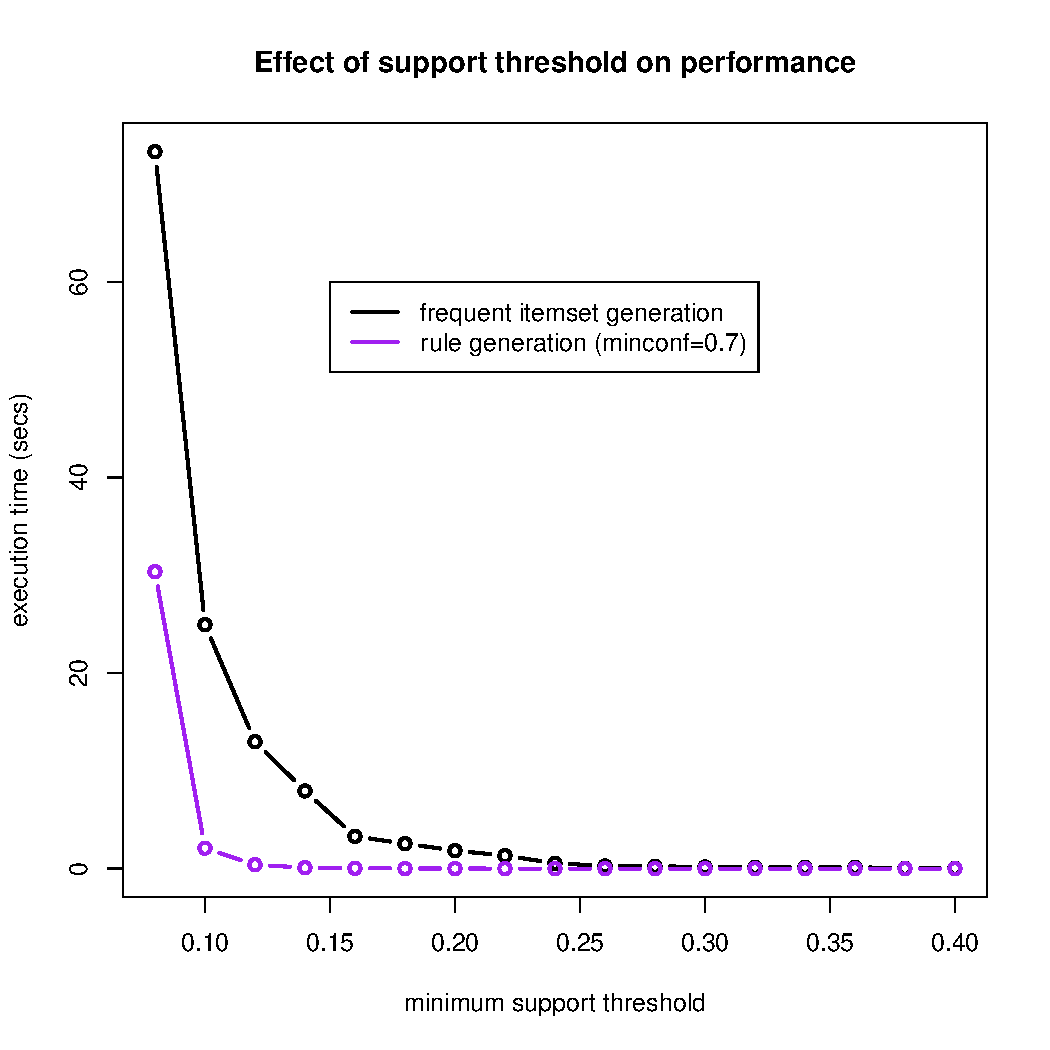
\includegraphics[scale=0.80]{plot1.pdf}
\end{figure}

\begin{figure}[H]
  \centering
  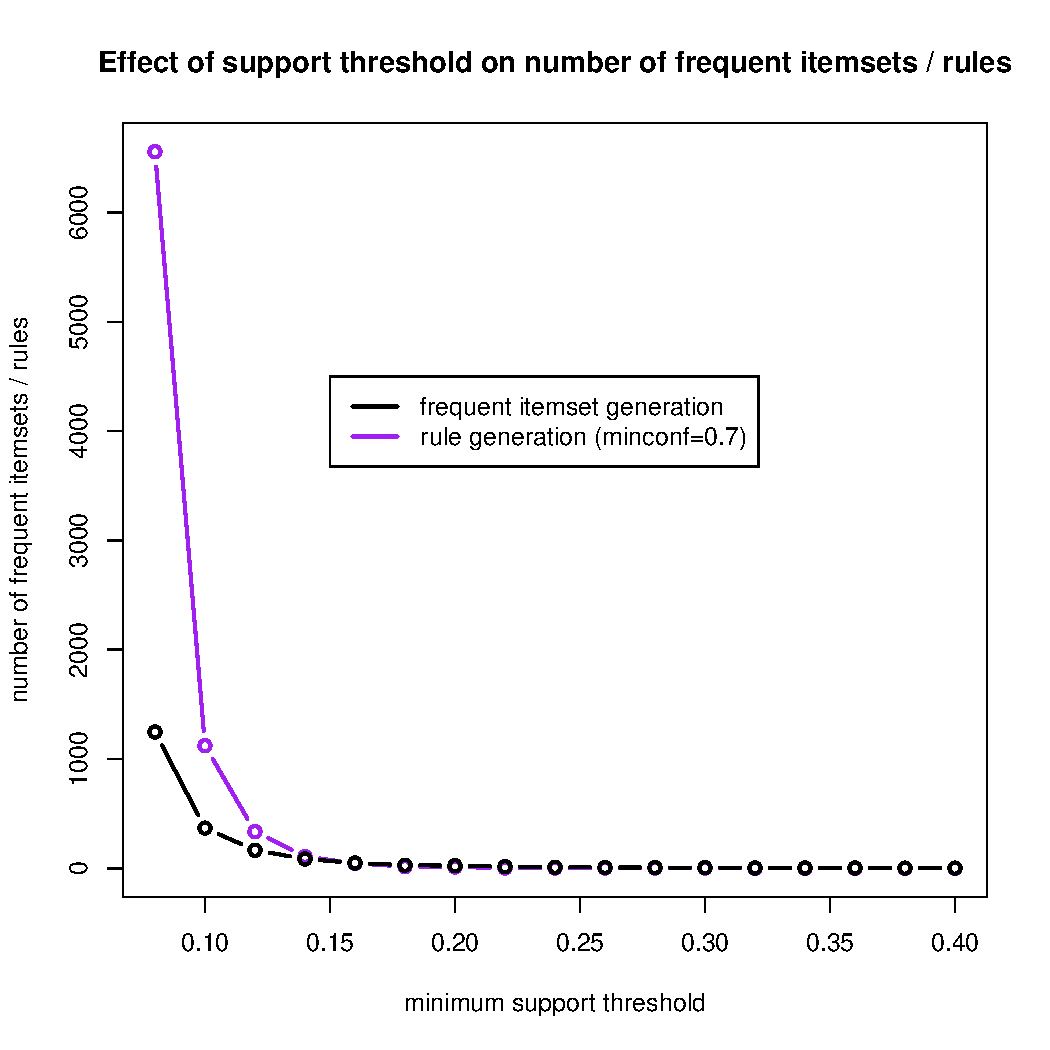
\includegraphics[scale=0.80]{plot2.pdf}
\end{figure}

\begin{figure}[H]
  \centering
  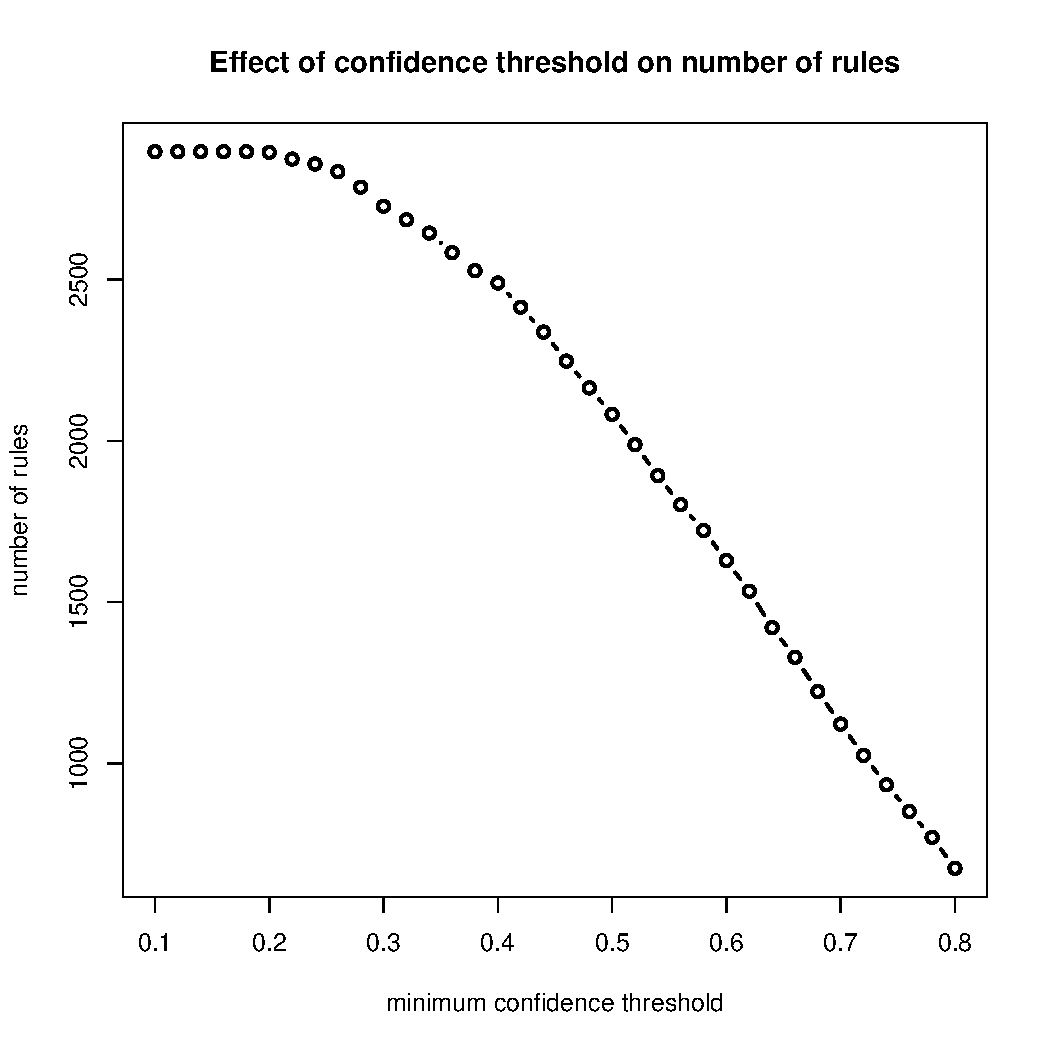
\includegraphics[scale=0.80]{plot3.pdf}
  \caption{Frequent itemsets obtained with $minsup = 0.10$, so a total of 368
  frequent itemsets beforehand.}
\end{figure}

I also tested the running times of different confidence thresholds but they
were so similar that I didn't bother wasting space plotting them. This is most
likely due to my inefficient implementation of rule generation, i.e. I always
generate all the rules first and prune them afterwards.

\section{Maximal frequent itemsets}
As I noticed that I still had some time to burn, I implemented maximal frequent
itemset generation as well. My implementation uses the results of Apriori's
frequent itemset generation procedure to its advantage.

Let's look at an example.
\begin{verbatim}
> freq.itemsets <- frequent.itemset.generation(mat, 0.2)

> freq.itemsets
[[1]]
[[1]]$itemsets
      [,1] 
 [1,] "131"
 [2,] "193"
 [3,] "52" 
 [4,] "77" 
 [5,] "80" 
 [6,] "83" 
 [7,] "84" 
 [8,] "85" 
 [9,] "86" 
[10,] "89" 
[11,] "91" 
[12,] "92" 

[[1]]$support.counts
 [1] 3487 2011 1865 2118 2436 4267 3129 1941 3166 2093 1696 1800


[[2]]
[[2]]$itemsets
      [,1]  [,2]
 [1,] "131" "83"
 [2,] "131" "84"
 [3,] "131" "86"
 [4,] "193" "86"
 [5,] "77"  "86"
 [6,] "80"  "86"
 [7,] "83"  "84"
 [8,] "83"  "86"
 [9,] "84"  "86"

[[2]]$support.counts
[1] 2547 1884 1903 1725 1766 1695 2554 2292 1971


[[3]]
[[3]]$itemsets
     [,1]  [,2] [,3]
[1,] "131" "83" "84"
[2,] "131" "83" "86"
[3,] "83"  "84" "86"

[[3]]$support.counts
[1] 1801 1732 1764



> maximal.frequent.itemsets(freq.itemsets)

[[1]]
[1] "52"

[[2]]
[1] "85"

[[3]]
[1] "89"

[[4]]
[1] "91"

[[5]]
[1] "92"

[[6]]
[1] "193" "86" 

[[7]]
[1] "77" "86"

[[8]]
[1] "80" "86"

[[9]]
[1] "131" "83"  "84" 

[[10]]
[1] "131" "83"  "86" 

[[11]]
[1] "83" "84" "86"
\end{verbatim}

The results tell us that e.g. itemsets $\{80, 86\}$ and $\{92\}$ are maximal
frequent. The R library "arules" gives the same results, so my implementation
should work correctly.

\section{What I learned}
One of the biggest lessons I learned is that it's definitely not trivial to
turn pseudocode into real runnable code. Much care must be taken to make sure
that things work correctly, and sometimes debugging can be very tedious. Even
after you have convinced yourself that your implementation works correctly,
you have the additional problem of performance.
\end{document}

% ---- EXAMPLES BELOW ----

% -- Example of figure for imagename.eps
% \begin{figure}
%     \includegraphics[scale=0.5]{imagename}
%     \caption*{Caption be here.}
% \end{figure}

% -- Example of floating figure for imagename.eps
% \begin{floatingfigure}[r]{0.49\textwidth}
%   \includegraphics[scale=0.31]{imagename}
%   \caption*{Caption be here.}
% \end{floatingfigure}

% -- Example of two figures side-by-side
% \begin{figure}[h]
%   \centering
%   \begin{subfigure}{.5\textwidth}
%     \centering
%     \includegraphics[width=.9\linewidth]{fig1.eps}
%     \caption*{Caption here}
%   \end{subfigure}%
%   \begin{subfigure}{.5\textwidth}
%     \centering
%     \includegraphics[width=.9\linewidth]{fig2.eps}
%     \caption*{Caption be here}
%   \end{subfigure}
%   \caption{Shared caption}
%   \label{fig:fighere}
% \end{figure}

% -- Remove pagination
% \thispagestyle{empty}
% \pagestyle{empty}

% -- Example of code listing
%\lstinputlisting[language=Ruby, caption={file.rb}]{./file.rb}

% -- Example of cases-environment
% $$
% f(x) =
% \begin{cases}
%     x^2 & \text{if } x > 0 \\
%     0 & \text{otherwise } \\
% \end{cases}
% $$

% -- Example of multicolumn row in tabular environment
% \multicolumn{3}{|c|}{Cell spanning three columns}
